\documentclass{standalone}
\usepackage{tikz}
\usetikzlibrary{patterns, positioning}

\begin{document}
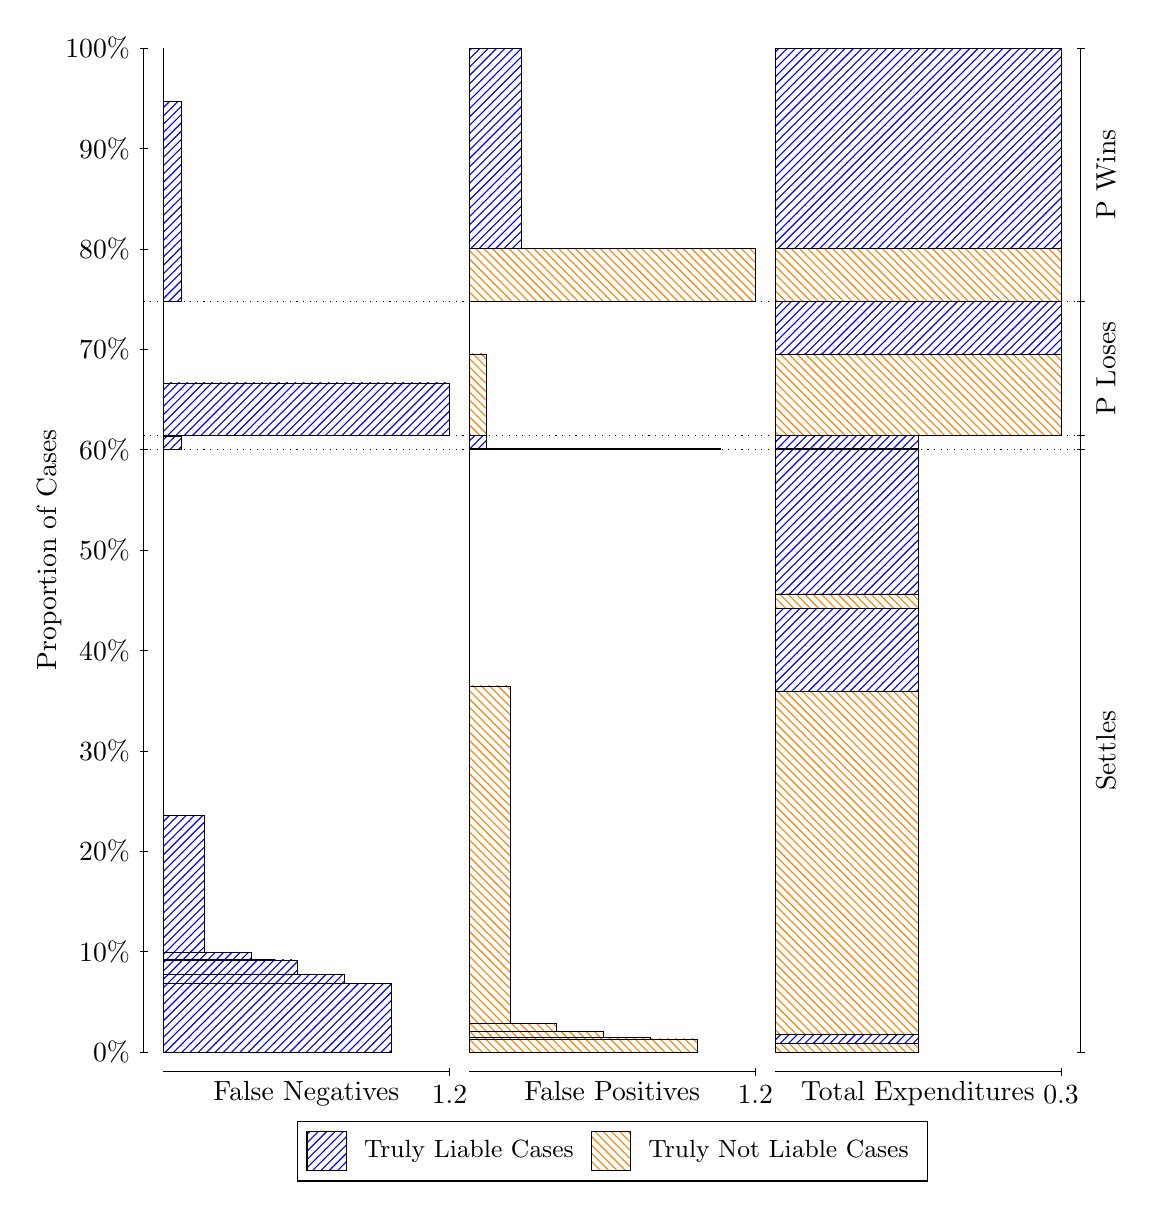
\begin{tikzpicture}
\draw[black, very thin] (1.5,1.75) -- (1.5,14.5);
\node[rotate=90, anchor=center] at (0.3, 8.125) {Proportion of Cases};
\draw[black, very thin] (1.45,1.75) -- (1.55,1.75);
\node[anchor=east] at (1.45, 1.75) {0\%};
\draw[black, very thin] (1.45,3.025) -- (1.55,3.025);
\node[anchor=east] at (1.45, 3.025) {10\%};
\draw[black, very thin] (1.45,4.3) -- (1.55,4.3);
\node[anchor=east] at (1.45, 4.3) {20\%};
\draw[black, very thin] (1.45,5.575) -- (1.55,5.575);
\node[anchor=east] at (1.45, 5.575) {30\%};
\draw[black, very thin] (1.45,6.85) -- (1.55,6.85);
\node[anchor=east] at (1.45, 6.85) {40\%};
\draw[black, very thin] (1.45,8.125) -- (1.55,8.125);
\node[anchor=east] at (1.45, 8.125) {50\%};
\draw[black, very thin] (1.45,9.4) -- (1.55,9.4);
\node[anchor=east] at (1.45, 9.4) {60\%};
\draw[black, very thin] (1.45,10.675) -- (1.55,10.675);
\node[anchor=east] at (1.45, 10.675) {70\%};
\draw[black, very thin] (1.45,11.95) -- (1.55,11.95);
\node[anchor=east] at (1.45, 11.95) {80\%};
\draw[black, very thin] (1.45,13.225) -- (1.55,13.225);
\node[anchor=east] at (1.45, 13.225) {90\%};
\draw[black, very thin] (1.45,14.5) -- (1.55,14.5);
\node[anchor=east] at (1.45, 14.5) {100\%};

\draw[black, very thin] (13.4,1.75) -- (13.4,14.5);
\draw[black, very thin] (13.35,1.75) -- (13.45,1.75);
\node[anchor=west] at (13.35, 1.75) {};
\draw[black, very thin] (13.35,9.4004) -- (13.45,9.4004);
\node[anchor=west] at (13.35, 9.4004) {};
\draw[black, very thin] (13.35,9.5799) -- (13.45,9.5799);
\node[anchor=west] at (13.35, 9.5799) {};
\draw[black, very thin] (13.35,11.283) -- (13.45,11.283);
\node[anchor=west] at (13.35, 11.283) {};
\draw[black, very thin] (13.35,14.5) -- (13.45,14.5);
\node[anchor=west] at (13.35, 14.5) {};

\draw[black, very thin, pattern color=blue, pattern=north east lines] (1.75,1.75) rectangle (4.6418,2.6234);
\draw[black, very thin, pattern color=blue, pattern=north east lines] (1.75,2.6234) rectangle (4.3452,2.626);
\draw[black, very thin, pattern color=blue, pattern=north east lines] (1.75,2.626) rectangle (4.0486,2.7375);
\draw[black, very thin, pattern color=blue, pattern=north east lines] (1.75,2.7375) rectangle (3.752,2.7403);
\draw[black, very thin, pattern color=blue, pattern=north east lines] (1.75,2.7403) rectangle (3.4554,2.9193);
\draw[black, very thin, pattern color=blue, pattern=north east lines] (1.75,2.9193) rectangle (3.1588,2.9215);
\draw[black, very thin, pattern color=blue, pattern=north east lines] (1.75,2.9215) rectangle (2.8622,3.0118);
\draw[black, very thin, pattern color=blue, pattern=north east lines] (1.75,3.0118) rectangle (2.269,4.7508);
\draw[black, very thin, pattern color=orange, pattern=north west lines] (1.75,4.7508) rectangle (1.75,9.4004);
\draw[black, very thin, pattern color=blue, pattern=north east lines] (1.75,9.4004) rectangle (1.9724,9.5639);
\draw[black, very thin, pattern color=orange, pattern=north west lines] (1.75,9.5639) rectangle (1.75,9.5799);
\draw[black, very thin, pattern color=blue, pattern=north east lines] (1.75,9.5799) rectangle (5.3833,10.247);
\draw[black, very thin, pattern color=orange, pattern=north west lines] (1.75,10.247) rectangle (1.75,11.283);
\draw[black, very thin, pattern color=blue, pattern=north east lines] (1.75,11.283) rectangle (1.9724,13.826);
\draw[black, very thin, pattern color=orange, pattern=north west lines] (1.75,13.826) rectangle (1.75,14.5);
\draw[black, very thin, pattern color=orange, pattern=north west lines] (5.6333,1.75) rectangle (8.5252,1.915);
\draw[black, very thin, pattern color=orange, pattern=north west lines] (5.6333,1.915) rectangle (7.932,1.934);
\draw[black, very thin, pattern color=orange, pattern=north west lines] (5.6333,1.934) rectangle (7.6354,1.9344);
\draw[black, very thin, pattern color=orange, pattern=north west lines] (5.6333,1.9344) rectangle (7.3388,2.0076);
\draw[black, very thin, pattern color=orange, pattern=north west lines] (5.6333,2.0076) rectangle (7.0422,2.0086);
\draw[black, very thin, pattern color=orange, pattern=north west lines] (5.6333,2.0086) rectangle (6.7456,2.1165);
\draw[black, very thin, pattern color=orange, pattern=north west lines] (5.6333,2.1165) rectangle (6.449,2.1175);
\draw[black, very thin, pattern color=orange, pattern=north west lines] (5.6333,2.1175) rectangle (6.1524,6.3996);
\draw[black, very thin, pattern color=blue, pattern=north east lines] (5.6333,6.3996) rectangle (5.6333,9.4004);
\draw[black, very thin, pattern color=orange, pattern=north west lines] (5.6333,9.4004) rectangle (8.8218,9.4164);
\draw[black, very thin, pattern color=blue, pattern=north east lines] (5.6333,9.4164) rectangle (5.8558,9.5799);
\draw[black, very thin, pattern color=orange, pattern=north west lines] (5.6333,9.5799) rectangle (5.8558,10.616);
\draw[black, very thin, pattern color=blue, pattern=north east lines] (5.6333,10.616) rectangle (5.6333,11.283);
\draw[black, very thin, pattern color=orange, pattern=north west lines] (5.6333,11.283) rectangle (9.2667,11.956);
\draw[black, very thin, pattern color=blue, pattern=north east lines] (5.6333,11.956) rectangle (6.3007,14.5);
\draw[black, very thin, pattern color=orange, pattern=north west lines] (9.5167,1.75) rectangle (11.333,1.8599);
\draw[black, very thin, pattern color=blue, pattern=north east lines] (9.5167,1.8599) rectangle (11.333,1.9768);
\draw[black, very thin, pattern color=orange, pattern=north west lines] (9.5167,1.9768) rectangle (11.333,6.3321);
\draw[black, very thin, pattern color=blue, pattern=north east lines] (9.5167,6.3321) rectangle (11.333,7.3845);
\draw[black, very thin, pattern color=orange, pattern=north west lines] (9.5167,7.3845) rectangle (11.333,7.5689);
\draw[black, very thin, pattern color=blue, pattern=north east lines] (9.5167,7.5689) rectangle (11.333,9.4004);
\draw[black, very thin, pattern color=orange, pattern=north west lines] (9.5167,9.4004) rectangle (11.333,9.4164);
\draw[black, very thin, pattern color=blue, pattern=north east lines] (9.5167,9.4164) rectangle (11.333,9.5799);
\draw[black, very thin, pattern color=orange, pattern=north west lines] (9.5167,9.5799) rectangle (13.15,10.616);
\draw[black, very thin, pattern color=blue, pattern=north east lines] (9.5167,10.616) rectangle (13.15,11.283);
\draw[black, very thin, pattern color=orange, pattern=north west lines] (9.5167,11.283) rectangle (13.15,11.956);
\draw[black, very thin, pattern color=blue, pattern=north east lines] (9.5167,11.956) rectangle (13.15,14.5);
\draw[black, dotted] (1.5,9.4004) -- (13.4,9.4004);
\draw[black, dotted] (1.5,9.5799) -- (13.4,9.5799);
\draw[black, dotted] (1.5,11.283) -- (13.4,11.283);
\draw[black, very thin] (1.75,1.5) -- (5.3833,1.5);
\node[anchor=north] at (3.5667, 1.5) {False Negatives};
\draw[black, very thin] (5.3833,1.45) -- (5.3833,1.55);
\node[anchor=north] at (5.3833, 1.45) {1.2};

\draw[black, very thin] (5.6333,1.5) -- (9.2667,1.5);
\node[anchor=north] at (7.45, 1.5) {False Positives};
\draw[black, very thin] (9.2667,1.45) -- (9.2667,1.55);
\node[anchor=north] at (9.2667, 1.45) {1.2};

\draw[black, very thin] (9.5167,1.5) -- (13.15,1.5);
\node[anchor=north] at (11.333, 1.5) {Total Expenditures};
\draw[black, very thin] (13.15,1.45) -- (13.15,1.55);
\node[anchor=north] at (13.15, 1.45) {0.3};

\node[black, centered, rotate=90] at (13.72, 5.5752) {Settles};

\node[black, centered, rotate=90] at (13.72, 10.431) {P Loses};
\node[black, centered, rotate=90] at (13.72, 12.891) {P Wins};

\draw (7.449999999999999,1.5) node[draw=none] (baseCoordinate) {};
\begin{scope}[align=center]
        \matrix[scale=0.5, draw=black, below=0.5cm of baseCoordinate, nodes={draw}, column sep=0.1cm]{
            \node[rectangle, draw, minimum width=0.5cm, minimum height=0.5cm, pattern=north east lines, pattern color=blue] {}; &
            \node[draw=none, font=\small] (B) {Truly Liable Cases}; &
            \node[rectangle, draw, minimum width=0.5cm, minimum height=0.5cm, pattern=north west lines, pattern color=orange] {}; &
            \node[draw=none, font=\small] (B) {Truly Not Liable Cases}; \\
            };
\end{scope}

\end{tikzpicture}
\end{document}